\documentclass{article}
\usepackage[utf8]{inputenc}
\usepackage{amsmath}
\usepackage{indentfirst}
\usepackage{graphicx,caption}
\usepackage[a4paper, margin=1in]{geometry}
\linespread{1.15}
\usepackage{empheq}
\usepackage[most]{tcolorbox}
\usepackage[margin=3cm]{caption}
\usepackage{siunitx}
\usepackage{array}
\usepackage{braket}
\usepackage{mathtools}

\usepackage{xcolor,sectsty}
\definecolor{astral}{RGB}{46,116,181}
\subsectionfont{\color{astral}}
\sectionfont{\color{astral}}

\title{
\includegraphics[width=0.1\textwidth]{ufallogo.png} \\
\Huge{\color{astral}\textbf{Teoria Quântica do Espalhamento}}}
\author{Paulo Brandão}
\date{Maio de 2017}

\newtcbox{\mymath}[1][]{%
    nobeforeafter, math upper, tcbox raise base,
    enhanced, colframe=blue!30!black,
    colback=blue!30, boxrule=1pt,
    #1}
\newcommand*{\bfrac}[2]{\genfrac{\lbrace}{\rbrace}{0pt}{}{#1}{#2}}
\begin{document}

\maketitle

\section{Introdução}

Com uma rápida pesquisa feita no site da instituição Nobel, é possível verificar que aproximadamente 60 prêmios Nobel foram dados para cientistas que trabalharam ou trabalham direta ou indiretamente com o assunto desta aula: Teoria Quântica do Espalhamento. Isso mostra o grau elevado de importância do tema. O objetivo desta seção introdutória é mostrar ao estudante um panorama geral da teoria a ser desenvolvida nas seções posteriores. Como o tema da aula tem um base muito forte do ponto de vista da física aplicada, é extremamente vantajoso divagar sobre certos aspectos gerais dos sistemas antes de nos aprofundarmos na teoria matemática em si.

\subsection{Descrição de Experimentos de Espalhamento}

A filosofia natural se preocupou por muito tempo em responder a pergunta: \textit{Como podemos explicar a imensa quantidade de fenômenos naturais em termos de substâncias primitivas e suas propriedades?} Na versão moderna, a pergunta seria formulada como: \textit{Quais são os constituintes primários da matéria e como eles interagem entre eles?} A resposta é obtida quase que exclusivamente através de experimentos de espalhamento. A teoria que relaciona os resultados de tais experimentos com as interações fundamentais existentes entre as partículas é chamada de \textbf{teoria do espalhamento}, que será o objetivo dessa aula. Sob esse ponto de vista fundamental da matéria, somos obrigados a considerar a interação entre as partículas num processo de espalhamento como regida pelas leis da mecânica quântica. Desse ponto de vista, estaremos voltados à teoria \textbf{quântica} do espalhamento.

Existe uma grande variedade de experimentos de espalhamento. No entanto, a grande maioria possui certos elementos em comum. As quatro partes essenciais de um experimento de espalhamento são: a \textbf{fonte S}, o \textbf{aparato preparador P}, o \textbf{alvo T} e o \textbf{detector D}, como mostra a representação esquemática na Fig. 1.

\begin{figure}[h]
\centering
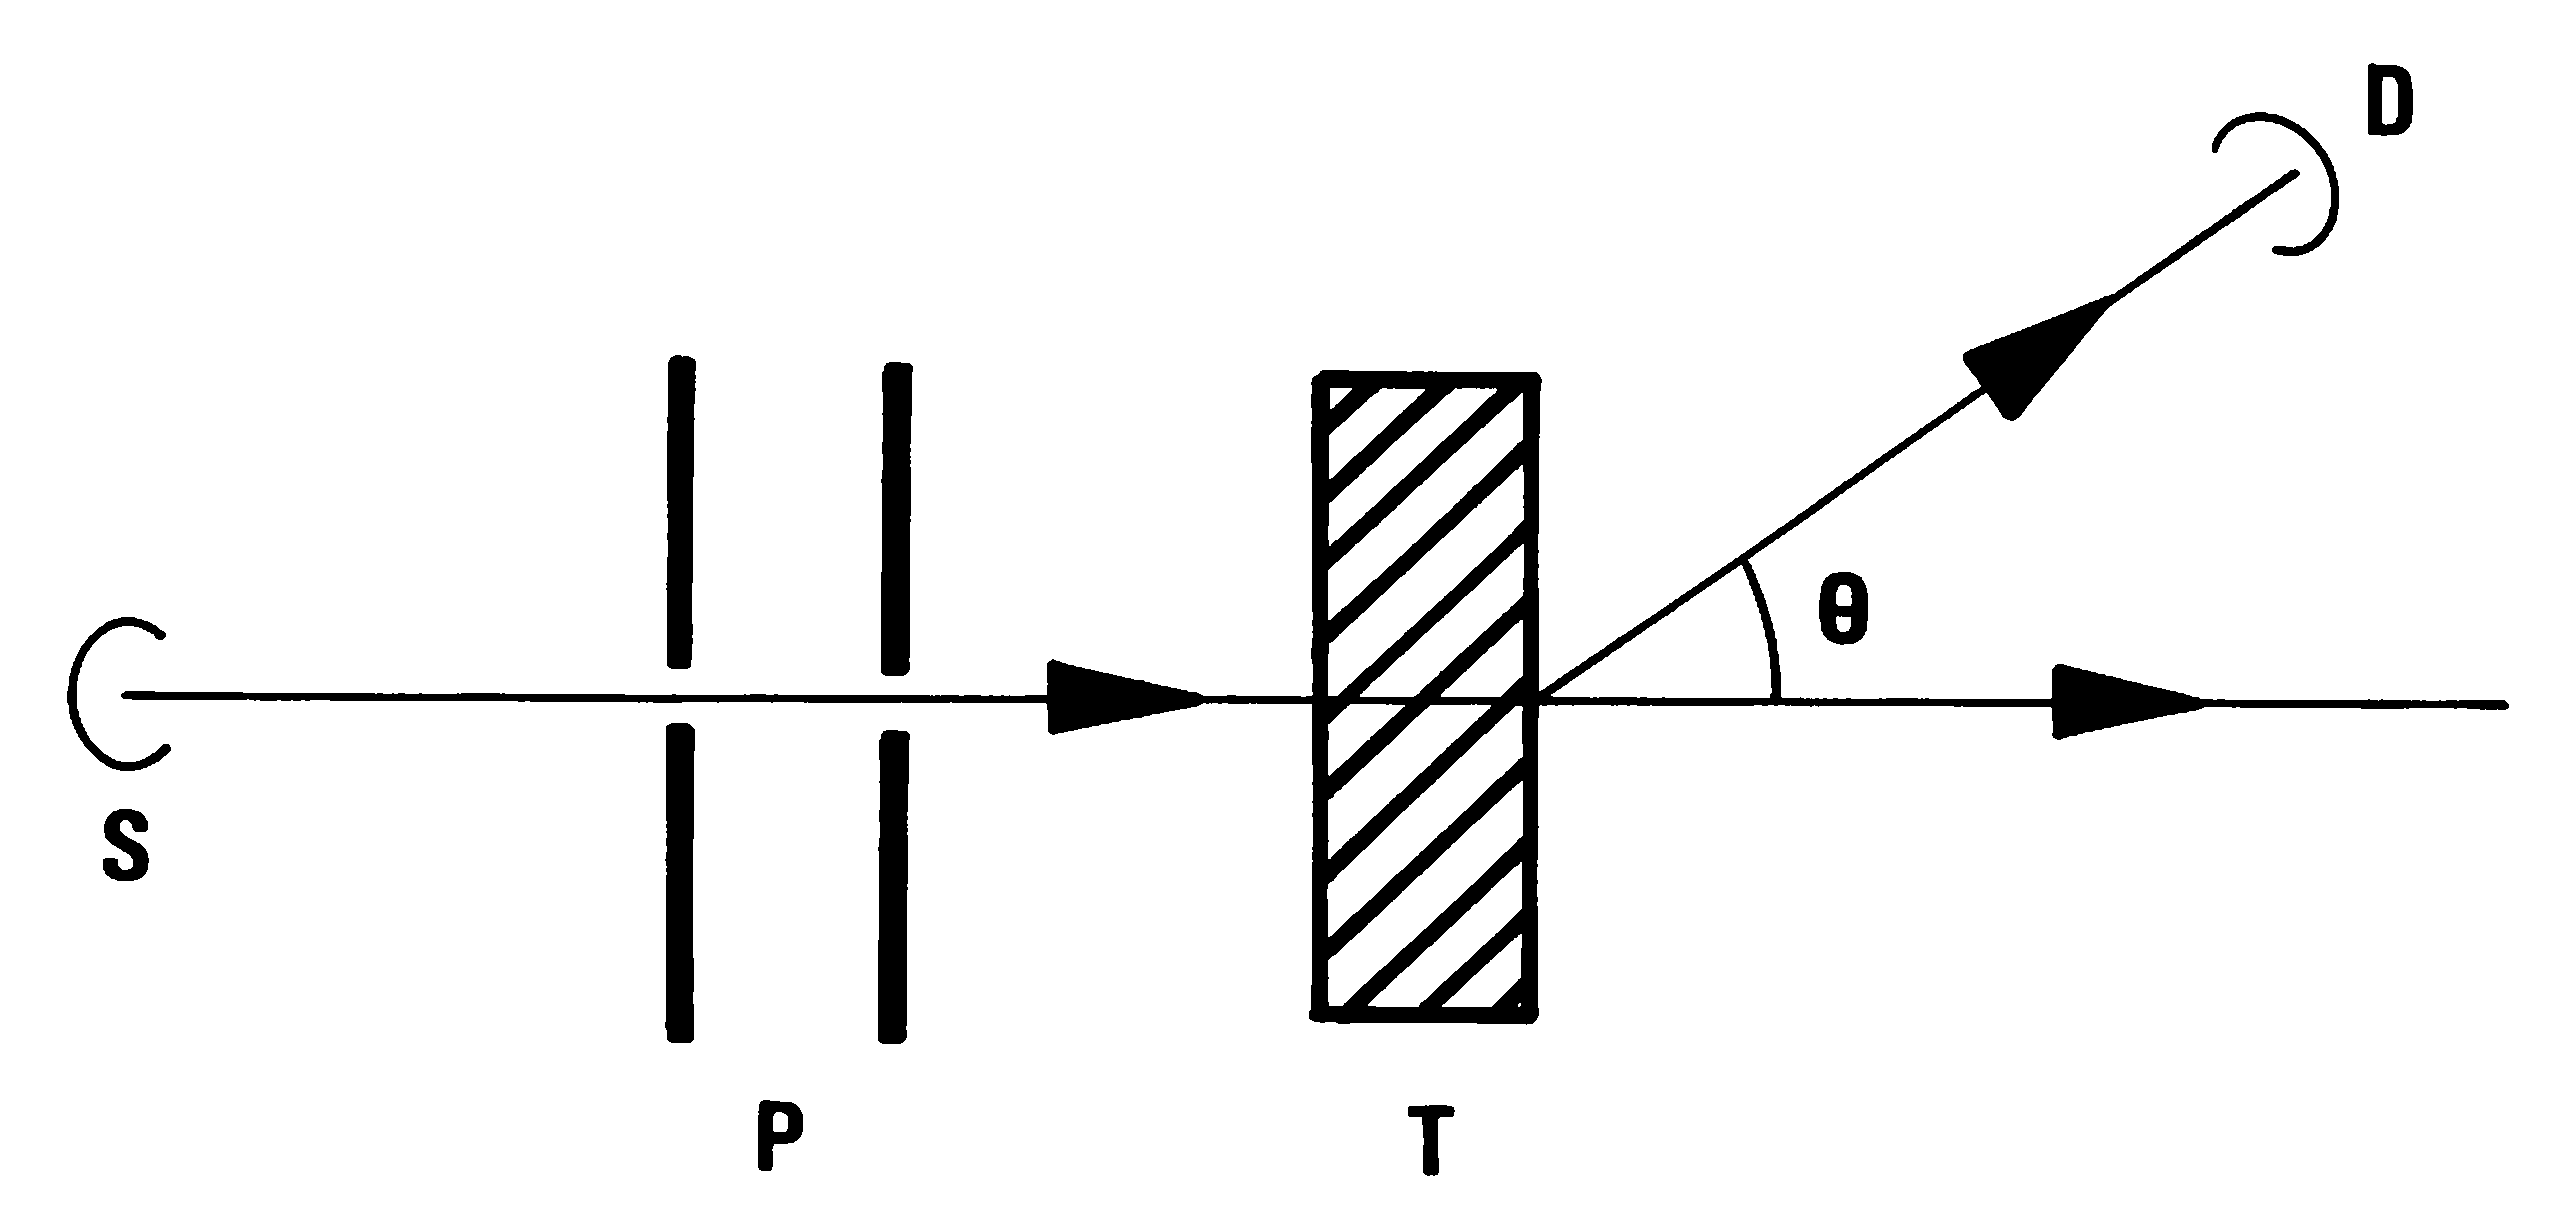
\includegraphics[width=8cm]{fig1.png}
\caption{Representação esquemática de um típico experimento de espalhamento. S é a fonte, P o aparato preparador, T o alvo e D o detector.}
\end{figure}

\noindent A fonte S produz as partículas que irão interagir com as partículas do alvo T. É importante que a fonte produza partículas sob condições praticamente idênticas e bem definidas. Lembre-se de que medidas em mecânica quântica são deitas considerando um grande número de sistemas idênticos (ensembles). O aparato preparador P pode ser um polarizador ou uma fenda para colimar as partículas provenientes da fonte S, por exemplo.

O alvo (ou amostra) T contém as partículas que supostamente irão interagir com as partículas incidentes. Se ou a amostra for relativamente grossa então \textbf{espalhamento múltiplo} pode ocorrer, que afeta a distribuição angular das partículas espalhadas. Se a amostra possuir uma estrutura cristalina, então efeitos de interferência serão importantes que também afetarão a distribuição angular. Se a amostra consistir de partículas em movimento (um gás), então efeitos importantes relativos ao movimento devem ser levados em conta.

O detector D é colocado numa posição de tal forma que ele detecta apenas as partículas espalhadas pelo alvo. Isto é, se o alvo for removido, o detector não pode ter uma resposta ao espalhamento. Na prática, isso pode ser bastante sutil de se realizar. É importante também que o detector seja colocado bastante longe do alvo de modo que uma partícula detectada não interaja mais com o alvo.


\subsection{Diferentes Tipos de Espalhamentos}

Podemos classificar os mais variados experimentos de espalhamento em duas classes: \textbf{elásticos} e \textbf{inelásticos}. O espalhamento elástico pode ser representado \textit{simbolicamente} por uma expressão do tipo
\begin{equation}
    \overbrace{\alpha + \beta}^{\text{Estado inicial}} \rightarrow \overbrace{\alpha + \beta}^{\text{Estado final}}.
\end{equation}
Essa expressão indica que as partículas $\alpha$ e $\beta$, no estado inicial, sofreram uma interação e foram espalhadas em partículas $\alpha$ e $\beta$ no estado final. O termo elástico se refere ao fato de que a energia cinética total antes do espalhamento tem o mesmo valor numérico da energia cinética total após o espalhamento. 

Quando as partículas da fonte e do alvo possuem graus internos de liberdade é possível que, após o espalhamento, uma das partículas (ou as duas) sofra uma mudança de energia interna. Por exemplo, podemos excitar um elétron para o estado excitado num átomo do alvo. Nesse caso, a energia cinética total antes do espalhamento é diferente da energia cinética total após a interação. O espalhamento é dito então \textbf{inelástico}.

Com energias muito altas, é possível criar novos tipos de partículas num experimento de espalhamento. Uma colisão entre duas partículas $\alpha$ e $\beta$, por exemplo, pode acontecer através do esquema mostrado na Fig. 2.

\begin{figure}[h]
\centering
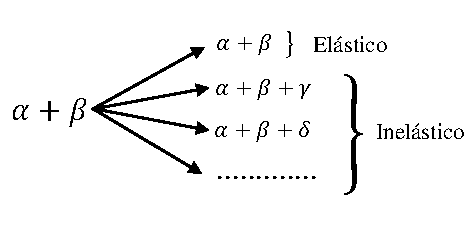
\includegraphics[width=8cm]{fig2.pdf}
\caption{Representação esquemática de um típico experimento de espalhamento onde novas partículas são criadas. }
\end{figure}

\noindent Para cada tipo de estado final possível num espalhamento chamamos de canal de espalhamento. Assim, na Fig. 2 temos um canal de espalhamento elástico e vários outros canais de espalhamento inelásticos. Se um Deutério (isótopo instável do Hidrogênio) interagir com um determinado potencial, podemos ter $d\rightarrow d$ ou $d\rightarrow p+n$ onde $p$ representa um próton e $n$ um nêutron, resultando assim em dois canais de espalhamentos possíveis onde o primeiro é elástico e o segundo inelástico. Nessa aula iremos tratar apenas de espalhamentos de canal único e elástico. Isto é, após a interação entre as duas partículas, obtemos as mesmas partículas (o alvo e a partícula espalhada) com energia total constante durante o movimento.

\subsection{Quantidades Observáveis}

O que realmente se mede num experimento de espalhamento? É claro que o detector irá medir um determinado número de partículas que foram absorvidas por ele através de uma área e por um período de tempo. Todas essas características estão codificadas na \textbf{seção de choque de espalhamento} que será introduzida mais na frente. O grande desafio do experimentalista é, com base nas direções e nas intensidades das partículas espalhadas pelo alvo, determinar as propriedades da amostra. De fato, foi através dos dados obtidos por um experimento de espalhamento de partículas alfa por folhas metálicas de ouro, que Rutherford inferiu a existência de um núcleo atômico.

No que segue, estaremos interessados apenas em espalhamento elástico descrito pela mecânica quântica não-relativística. Além disso, em geral, o tema de espalhamento é encontrado em livros-texto de forma dividida. Numa primeira análise, a teoria é demonstrada através da transmissão e reflexão de pacotes de ondas por potenciais do tipo "degrau". Coeficientes de transmissão e reflexão são calculados e representam as probabilidades da partícula ser transmitida através do potencial ou ser refletida pelo mesmo. No entanto, nesta aula, iremos considerar o problema de espalhamento do ponto de vista mais geral e mais aplicado à sistemas reais. Esse tema é geralmente tratado no final dos cursos de teoria quântica na graduação.


\section{Formalismo do Espalhamento Quântico}

A quantidade mais importante numa teoria de espalhamento é a seção de choque diferencial. É através dela que conseguimos obter informações acerca do alvo a ser estudado. Antes de introduzir a seção de choque no contexto da mecânica quântica, vamos compreender sua definição em um problema clássico com o objetivo de ganhar uma intuição mais aprofundada sobre essa grandeza. Dessa forma, considere uma partícula clássica sendo espalhada por um alvo localizado na origem do sistema de coordenadas, como ilustra a Fig. 3. Se a partícula passar pela área $d\sigma$, será espalhada por um ângulo sólido $d\Omega$. A razão entre essas duas quantidades é chamada de \textbf{seção de choque diferencial} $D(\theta,\phi)$:
\begin{empheq}[box=\tcbhighmath]{equation}
    D(\theta) = \frac{d\sigma}{d\Omega}.
\end{empheq}
A seção de choque \textbf{total} é obtida através da integração da seção de choque diferencial através do ângulo sólido: $D_{t} = \int D(\theta)d\Omega = \int (d\sigma/d\Omega) d\Omega$. Note que a dimensão da seção de choque é de área e que assumimos que o espalhamento ocorre para um ângulo $\phi$ (coordenada azimutal esférica) constante. Isto é, o alvo não pode espalhar a partícula para fora do plano da figura. 

\begin{figure}[h]
\centering
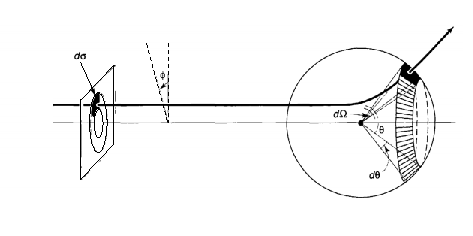
\includegraphics[width=8cm]{fig3.pdf}
\caption{Partículas incidentes na área $d\sigma$ são espalhadas dentro do ângulo sólido $d\Omega$}
\end{figure}

Agora que sabemos a grandeza importante que pode ser medida em laboratórios, a seção de choque diferencial (total), nosso objetivo é relacionar esta quantidade com as grandezas da teoria quântica, isto é, a função de onda. Esse tema é bastante complexo e, como foi discutido na introdução, existem vários níveis de aproximação. Iremos considerar apenas colisões elásticas entre duas partículas onde o potencial sentido pela partícula incidente depende apenas da distância $r$ (e não dos ângulos esféricos) com relação ao alvo. Dessa forma, a trajetória do objeto espalhado se dará no mesmo plano da trajetória incidente. Existem basicamente dois formalismos para se resolver a equação de Schrödinger nessa situação. A expansão em ondas parciais e as aproximações de Born. No que segue, iremos tratar apenas do método de Born. O aluno interessado em aprender outros métodos mais sofisticados pode consultar as referências presentes no plano de Aula. Para o que estamos interessados em demonstrar, o método de Born é suficiente.

Nosso objetivo é portanto resolver a equação de Schrödinger independente do tempo
\begin{equation}
    -\frac{\hbar^2}{2m}\nabla^2\psi(\mathbf{r}) + V(\mathbf{r})\psi(\mathbf{r}) = E\psi(\mathbf{r})
\end{equation}
ou
\begin{equation}
    (\nabla^2 + k^2)\psi(\mathbf{r}) = Q(\mathbf{r})
\end{equation}
onde
\begin{equation}
    k = \frac{\sqrt{2mE}}{\hbar} \hspace{1cm} Q(\mathbf{r}) = \frac{2m}{\hbar^2}V(\mathbf{r})\psi(\mathbf{r}).
\end{equation}
Note que a função de onda (que queremos calcular para um determinado potencial $V$) aparece implicitamente no lado direito da Eq. (4) através da definição da função $Q$. O método de solução da equação (4) é descrito no Apêndice.



A solução da Eq. (3) é portanto
\begin{empheq}[box=\tcbhighmath]{equation}
    \psi(\mathbf{r}) = \psi_0 (\mathbf{r}) - \frac{m}{2\pi\hbar^2}\int\frac{e^{ik|\mathbf{r}-\mathbf{r}'|}}{|\mathbf{r}-\mathbf{r}'|}V(\mathbf{r}')\psi(\mathbf{r}')d^{3}\mathbf{r}'
\end{empheq}
onde $\psi_0(\mathbf{r})$ satisfaz a equação de Helmholtz com $V = 0$: $(\nabla^2 + k^2)\psi_0(\mathbf{r}) = 0$. A Eq. (6) é a \textit{forma integral da equação de Schrödinger}, completamente equivalente à forma diferencial e, no caso do espalhamento, muito mais conveniente, como veremos. Cuidado! A função de onda $\psi$ aparece dentro da integral e, portanto, uma simples integração não pode ser feita porque não conhecemos o integrando. Como podemos proceder?











\section{Aproximação de Born}

Vamos supor que a energia potencial criada pelo alvo $V(\mathbf{r}')$ tem um alcance limitado de tal forma que $V = 0$ fora de uma região finita e que nosso objetivo é calcular a função de onda $\psi(\mathbf{r})$ em pontos muito distantes do espalhador. Nessas condições podemos escrever $|\mathbf{r}| \gg |\mathbf{r}'|$ de tal forma que o denominador na integral pode ser aproximado por
\begin{equation}
    |\mathbf{r}-\mathbf{r}'| \approx r - \hat{r}\cdot\mathbf{r}'
\end{equation}
onde $r = |\mathbf{r}|$ e $\hat{r} = \mathbf{r}/r$. Seja  $\mathbf{k} = k\hat{r}$, então
\begin{equation}
    e^{ik|\mathbf{r}-\mathbf{r}'|} \approx e^{ikr}e^{-i\mathbf{k}\cdot\mathbf{r}'}
\end{equation}
e
\begin{equation}
    \frac{e^{ik|\mathbf{r}-\mathbf{r}'|}}{|\mathbf{r}-\mathbf{r}'|} \approx \frac{e^{ikr}}{r}e^{-i\mathbf{k}\cdot\mathbf{r}'}
\end{equation}
de modo que a forma integral (6) fica
\begin{equation}
    \psi(\mathbf{r}) = \psi_0 (\mathbf{r}) - \frac{m}{2\pi\hbar^2}\frac{e^{ikr}}{r}\int e^{-i\mathbf{k}\cdot\mathbf{r}'} V(\mathbf{r}')\psi(\mathbf{r}')d^{3}\mathbf{r}'   . 
\end{equation}
A função de onda $\psi$ ainda se encontra dentro da integral apesar de todas as aproximações feitas até aqui. É nesse ponto que entra a primeira aproximação de Born. Born assumiu que a onda incidente, representada pela função $\psi_0$, não é \textit{substancialmente alterada} pela presença do potencial $V$. Assim, se a onda incidente for uma onda plana propagando-se na direção $\mathbf{k}'$, 
\begin{equation}
    \psi_0(\mathbf{r}) = Ae^{i\mathbf{k}'\cdot\mathbf{r}},
\end{equation}
onde $A$ é uma constante, então
\begin{equation}
\begin{split}
\psi(\mathbf{r}) &= \psi_0 (\mathbf{r}) - \frac{m}{2\pi\hbar^2}\frac{e^{ikr}}{r}\int e^{-i\mathbf{k}\cdot\mathbf{r}'} V(\mathbf{r}')\psi(\mathbf{r}')d^{3}\mathbf{r}' \\
                 &\approx \psi_0 (\mathbf{r}) - \frac{m}{2\pi\hbar^2}\frac{e^{ikr}}{r}\int e^{-i\mathbf{k}\cdot\mathbf{r}'} V(\mathbf{r}')\psi_0(\mathbf{r}')d^{3}\mathbf{r}' \\
                 &\approx \psi_0(\mathbf{r})+f(\theta,\phi)\frac{e^{ikr}}{r}
\end{split}
\end{equation}
onde a função
\begin{empheq}[box=\tcbhighmath]{equation}
f(\theta,\phi) = - \frac{m}{2\pi\hbar^2}\int V(\mathbf{r}')e^{i(\mathbf{k}'-\mathbf{k})\cdot\mathbf{r}'}d^{3}\mathbf{r}'
\end{empheq}
é chamada de \textbf{amplitude de espalhamento}. O final da Eq. (12) representa a soma de duas ondas. O primeiro termo é simplesmente a onda incidente no alvo e o segundo termo tem a forma de uma onda esférica cuja amplitude é modulada nos ângulos $\phi$ e $\theta$ através da função $f$ que, por sua vez, depende do potencial espalhador $V$! A Eq. (13) mostra que a função $f$ é a transformada de Fourier do potencial $V(\mathbf{r})$ na variável de momento $\mathbf{s} = \mathbf{k}'-\mathbf{k}$. Como assumimos que o potencial é praticamente nulo fora de uma determinada região, sua transformada de Fourier existe (assumindo que a função também é contínua).

Para um potencial radial, isto é, que depende apenas da distância $r$, $V(\mathbf{r}) = V(|\mathbf{r}|) = V(r)$ podemos definir
\begin{equation}
    \mathbf{u} = \mathbf{k}'-\mathbf{k}
\end{equation}
e como $d^3 \mathbf{r}' = (r')^2\sin\theta' d\theta' d\phi'$ podemos escrever
\begin{equation}
f(\theta,\phi) = - \frac{m}{2\pi\hbar^2}\int V(r')e^{i\mathbf{u}\cdot\mathbf{r}'}(r')^2\sin\theta' d\theta' d\phi'.
\end{equation}
Se escolhermos o eixo polar das variáveis de integração em coordenadas esféricas na direção de $\mathbf{u}$, então $\mathbf{u}\cdot\mathbf{r}' = ur' \cos\theta'$. A integral em $\phi$ vale $2\pi$ e ficamos com
\begin{equation}
f(\theta,\phi) = - \frac{m}{\hbar^2}\int V(r')e^{iur'\cos\theta'}(r')^2\sin\theta' d\theta'.    
\end{equation}
A integral em $\theta'$ é dada por
\begin{equation}
    \int_{0}^{\pi} e^{iyz\cos x}\sin x dx = \frac{2\sin(yz)}{yz}
\end{equation}
resultando em
\begin{empheq}[box=\tcbhighmath]{equation}
    f(\theta) = -\frac{2m}{\hbar^2 u}\int_0^{\infty} rV(r)\sin(ur)dr
\end{empheq}
onde $u = 2k\sin(\theta/2)$ como pode ser facilmente verificado.

\subsection{Relação Entre $f$ e a Seção de Choque}

Para finalizar nossa análise, basta encontrarmos a relação entre a função amplitude $f(\theta)$ e a seção de choque diferencial $d\sigma/d\Omega$. Feito isso, é possível calcular os ângulos de espalhamento após especificarmos um potencial radial $V(r)$, que é o objetivo principal desta aula.

Em primeiro lugar, não podemos utilizar o conceito de trajetória na descrição quântica do movimento de uma partícula, como é empregado na mecânica clássica, pois uma única partícula é descrita por uma função de onda $\psi(\mathbf{r},t)$ que se estende pelo espaço. Dessa forma, a descrição do espalhamento terá uma natureza probabilística. Com relação à Fig. 3, devemos falar na probabilidade da partícula atravessar um volume de área transversal $d\sigma$ e altura $vdt$ e ser detectada no outro volume de área $dA$ e altura $dr$ próximo ao detector, como ilustra a Figura 4.

\begin{figure}[h]
\centering
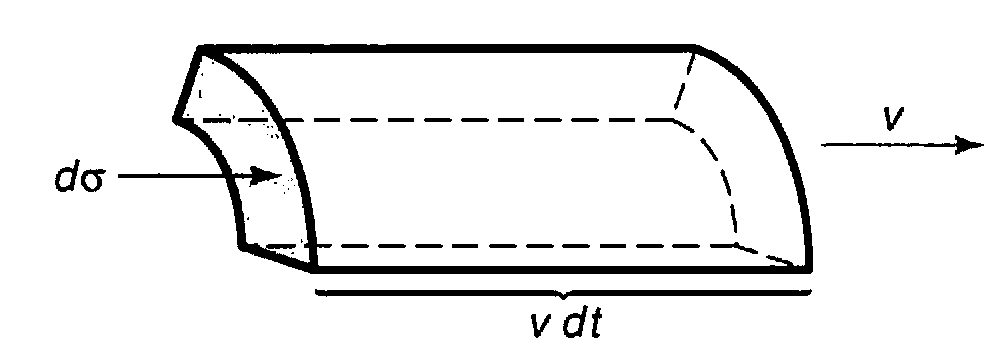
\includegraphics[width=8cm]{fig4.png}
\caption{O volume $dV$ do feixe incidente que passa pela área $d\sigma$ no tempo $dt$.}
\end{figure}

Assim, uma partícula incidente tem uma probabilidade $dP$ de ser detectada no volume $dV$ dada por
\begin{equation}
    dP = |\psi_\text{incidente}|^{2} dV = |A|^2 (vdt)d\sigma
\end{equation}
que é igual à probabilidade da partícula ser espalhada no ângulo sólido correspondente $d\Omega$
\begin{equation}
    dP = |\psi_\text{espalhada}|^2 dV = \frac{|A|^2 |f|^2}{r^2} (vdt)r^2 d\Omega
\end{equation}
ou
\begin{equation}
    |A|^2 (vdt)d\sigma = \frac{|A|^2 |f|^2}{r^2} (vdt)r^2 d\Omega
\end{equation}
\begin{equation}
    d\sigma = \frac{|f|^2}{r^2}r^2 d\Omega
\end{equation}
\begin{equation}
    d\sigma = |f|^2 d\Omega
\end{equation}
ou
\begin{equation}
    D(\theta) = |f(\theta)|^2.
\end{equation}
Concluímos que o módulo ao quadrado da amplitude de espalhamento é a seção de choque transversal do nosso problema. Explicitamente, a seção de choque é escrita como
\begin{empheq}[box=\tcbhighmath]{equation}
    D(\theta) = \frac{m^2}{\hbar^2 k^2 \sin^{2}(\theta/2)} \left| \int_{0}^{\infty} r V(r) \sin\left[ 2k\sin\left( \frac{\theta}{2} \right) r \right] dr \right|^{2}
\end{empheq}


\section{Aplicações}

\subsection{Potencial ``Esfera Rígida''}

Estamos prontos para calcular alguns tipos de espalhamentos. Vamos considerar inicialmente que o potencial criado pelo alvo existe em apenas uma esfera de raio $a$ ao redor do espalhador e possui valor $V_0$. Fora dessa esfera o potencial é nulo e a partícula incidente não sente a ação de nenhuma força nessa região. Ou seja, estamos interessados numa função potencial $V(r)$ tal que
\[
 V(r) = 
  \begin{cases} 
   V_0 & \text{if } r \leq 0 \\
   0       & \text{if } x > 0
  \end{cases}
\]
como ilustra a Figura 5. O primeiro passo é calcular a integral da Eq. (25). Ela é facilmente resolvida:

\begin{equation}
\int_{0}^{\infty} r V(r) \sin\left( u r \right) dr=V_0 \int_0^{a}r \sin(ur) dr = \frac{V_0}{u^2} \left[ \sin (au)-au\cos (au) \right]
\end{equation}
de forma que
\begin{equation}
D(\theta) = \frac{4m^2 V_0^2}{\hbar^2 u^6}|\sin(au) - au\cos(au)|^2    
\end{equation}
com $u = 2k\sin(\theta/2)$. A Figura 6 mostra o gráfico da função $D(\theta)$ em função do ângulo de espalhamento. É fácil ver pelo gráfico que a distribuição do espalhamento, isto é, a probabilidade de encontrar a partícula num determinado ângulo sólido numa posição angular $\theta$, é praticamente constante. Existe uma pequena queda na direção perpendicular à onda incidente.

\begin{figure}[h]
\centering
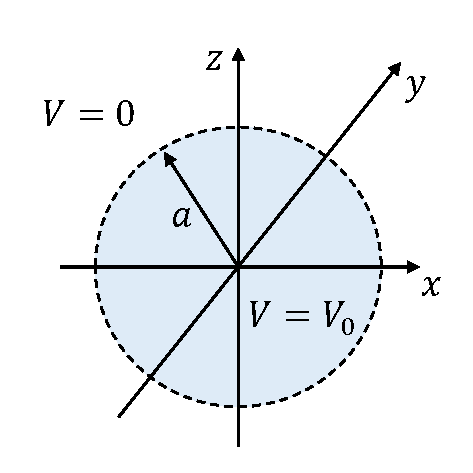
\includegraphics[width=5cm]{fig5.pdf}
\caption{Nessa situação, o potencial $V(r)$ é uma constante $V_0$ para $r\leq a$ e nulo para $r>0$.}
\end{figure}

\begin{figure}[h]
\centering
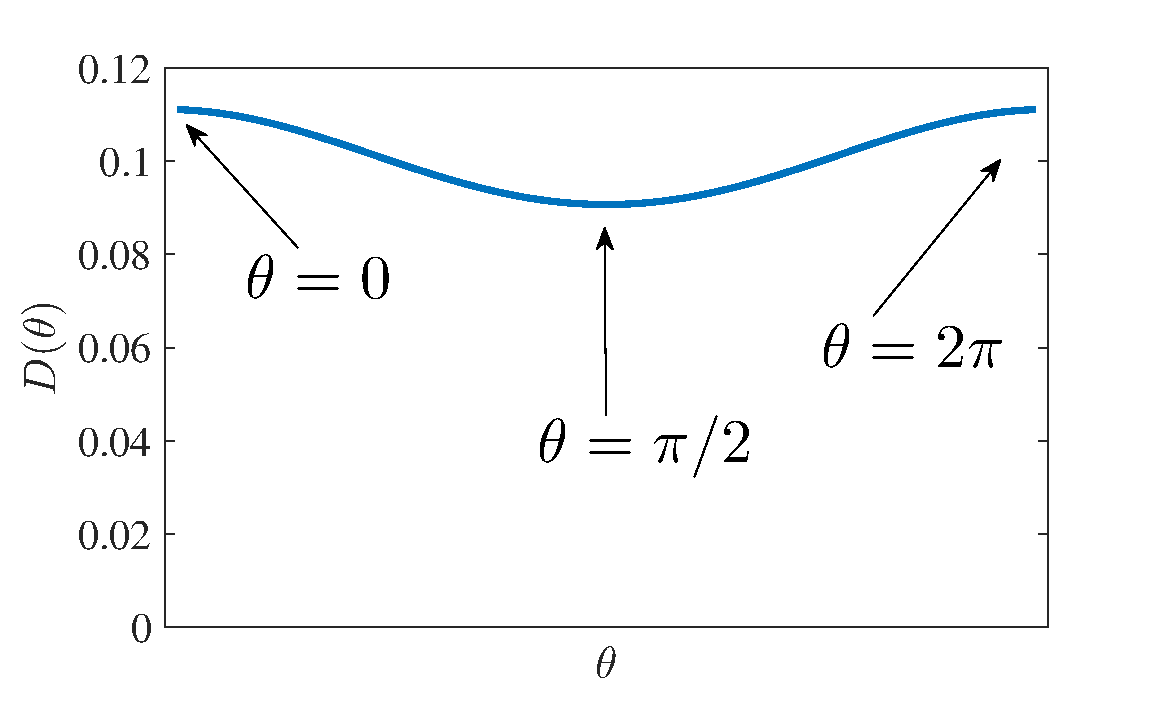
\includegraphics[width=6cm]{fig6.eps}
\caption{Seção de choque diferencial para o espalhamento de uma partícula quântica por um potencial do tipo ``esfera rígida''. Os valores utilizados foram apenas para ilustração: $k = 1$, $m = 1$, $\hbar = 1$, $V_0 = 1$ e $a = 1$.}
\end{figure}

\subsection{Potencial de Yukawa}

O potencial de Yukawa representa uma modelo grosseiro para a força de atração num núcleo atômico dada por
\begin{equation}
    V(r) = \beta\frac{e^{-\mu r}}{r}
\end{equation}
onde $\beta$ e $\mu$ são constantes. A integral necessária para calcular a amplitude de espalhamento vale agora
\begin{equation}
\int_{0}^{\infty} r V(r) \sin\left( u r \right) dr = \beta\int_0^{\infty} e^{-\mu r}\sin(ur)dr,   
\end{equation}
mas é fácil verificar que
\begin{equation}
    \int_0^{\infty}e^{-a x}\sin(bx) dx = \frac{b}{a^2 + b^2} \hspace{0.5cm} (a\geq 0),
\end{equation}
como $\mu>0$ então
\begin{equation}
\int_{0}^{\infty} r V(r) \sin\left( u r \right) dr =   \frac{\beta u}{\mu^2 + u^2}.  
\end{equation}
A seção de choque diferencial é dada por
\begin{equation}
    D(\theta) = \frac{4m^2}{\hbar^2 u^2} \left| \frac{\beta u}{\mu^2 + u^2} \right|^{2} = \frac{4 m^2 \beta^2}{\hbar^2} \frac{1}{\mu^2 + u^2} = \frac{4 m^2 \beta^2}{\hbar^2} \frac{1}{\mu^2 + 4k^2 \sin^2 (\theta/2)}.
\end{equation}
O gráfico da seção de choque diferencial está mostrado na Figura 7.

\begin{figure}[h]
\centering
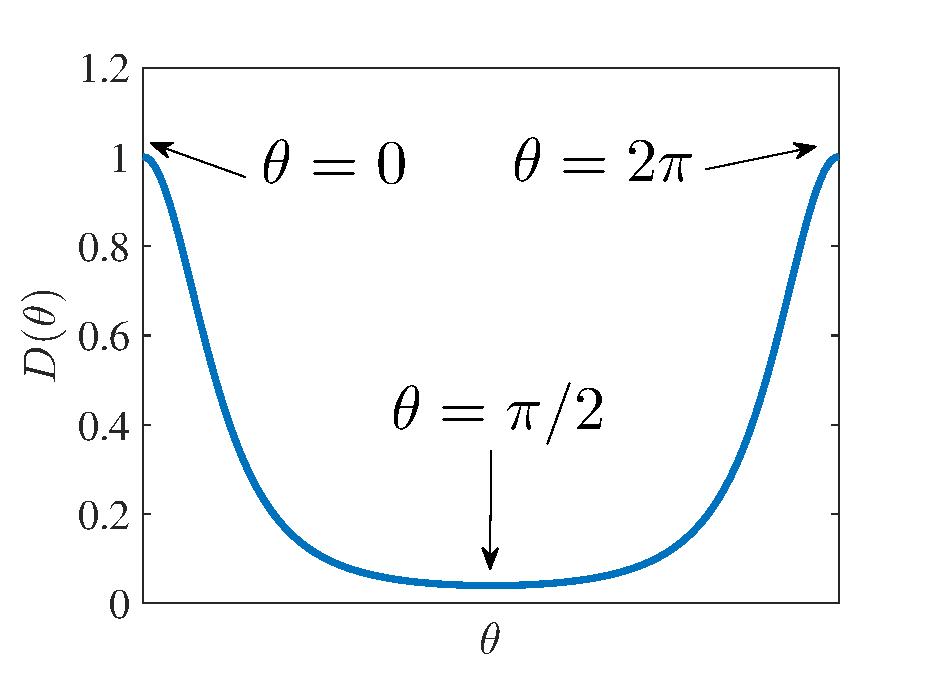
\includegraphics[width=6cm]{fig7.eps}
\caption{Seção de choque diferencial para o espalhamento de uma partícula quântica por um potencial Yukawa. Os valores utilizados foram apenas para ilustração: $k = 1$, $m = 1$, $\hbar = 1$, $\mu = 1$ e $\beta = 1$.}
\end{figure}

\subsection{Potencial de Coulomb (Espalhamento de Rutherford)}

Se tomarmos $\mu = 0$ e $\beta = q_1 q_2 /4\pi\varepsilon_0$, o potencial de Yukawa se torna o potencial Coulombiano, descrevendo a interação entre duas cargas $q_1$ e $q_2$. Pela substituição direta desses valores na Eq. (32) obtemos a seção de choque diferencial 
\begin{equation}
    D(\theta) = \left[ \frac{q_1 q_2}{16 \pi \varepsilon_0 E \sin^2 (\theta/2)} \right]^2
\end{equation}
onde $E = \hbar^2 k^2 /2m$ é a energia da partícula. Curiosamente, o mesmo resultado é obtido através da mecânica \textbf{clássica}.

\section{Aproximação de Born Para Altas Ordens}

Vamos reescrever a Eq. (6) na seguinte forma
\begin{equation}
    \psi(\mathbf{r}) = \psi_0 (\mathbf{r}) - \int g(\mathbf{r}-\mathbf{r}')V(\mathbf{r}')\psi(\mathbf{r}')d^3 {\mathbf{r}}'.
\end{equation}
Substitua a função $\psi_{\mathbf{r}}$ dentro da própria equação para obter
\begin{equation}
    \psi(\mathbf{r}) = \psi_0 (\mathbf{r}) - \int g(\mathbf{r}-\mathbf{r}')V(\mathbf{r}')\psi_0(\mathbf{r}')d^3 {\mathbf{r}}' + \int\int g(\mathbf{r}-\mathbf{r}')V(\mathbf{r}')g(\mathbf{r}''-\mathbf{r}')V(\mathbf{r}'') \psi (\mathbf{r}'') d^3 {\mathbf{r}}'d^3 {\mathbf{r}}''.
\end{equation}
É fácil ver que o primeiro termo do lado direito da Eq. (35) representa a solução do problema sem o potencial $V$. Esse termo é a ordem zero da solução. O segundo termo é a primeira ordem da expansão de Born e foi com ele que nos preocupamos durante toda a aula. Se aplicarmos novamente a função de onda (34) na (35) obteremos as ordens mais altas da aproximação e assim por diante. Geralmente não calculamos mais do que dois termos nessa expansão pelo motivo óbvio de que elas ficam cada vez mais complicadas.


\section{Conclusão}

A aproximação de Born é apenas um dos mais variados métodos para tratar espalhamento em sistemas quânticos. Tocamos aqui apenas na superfície dessa intensa e muito importante área de pesquisa. Tratamentos mais especializados podem ser encontrados nas referências no plano de aula fornecido.




\section*{Apêndice:  Solução da Equação $(\nabla^2 + k^2)\psi = Q$}

Suponha que resolvemos a equação não-homogênea de Helmholtz porém com o termo não homogêneo dado pela função delta de Dirac (e chame essa solução de $G$):
\begin{equation}
    (\nabla^2 + k^2)G(\mathbf{r}) = \delta(\mathbf{r}). 
\end{equation}
Se tivermos sucesso em encontrar $G$, então obtemos a solução do problema para $\psi$
\begin{equation}
    \psi(\mathbf{r}) = \int G(\mathbf{r}-\mathbf{r}')Q(\mathbf{r}')d^3 \mathbf{r}'
\end{equation}
pois
\begin{equation}
    (\nabla^2 + k^2)\psi(\mathbf{r}) = \int \left[ (\nabla^2 + k^2)G(\mathbf{r}-\mathbf{r}')Q(\mathbf{r}') \right]d^3 \mathbf{r}' = \int \delta (\mathbf{r}-\mathbf{r}')Q(\mathbf{r}')d^3 \mathbf{r}' = Q(\mathbf{r}).
\end{equation}
A função $G$ é chamada de \textit{função de Green} do sistema. Ela representa a resposta (ou solução) do sistema quando a fonte (lado direito não-homogêneo da equação) é uma delta de Dirac. A maneira mais fácil de resolver a equação de Helmholtz não-homogênea é utilizando a transformada de Fourier da função de Green,
\begin{equation}
    G(\mathbf{r}) = \frac{1}{(2\pi)^{3/2}}\int e^{i\mathbf{s}\cdot\mathbf{r}}g(\mathbf{s}) d^3 \mathbf{s},
\end{equation}
e a transformada de Fourier da função delta,
\begin{equation}
    \delta^3 (\mathbf{r}) = \frac{1}{(2\pi)^{3/2}}\int e^{i\mathbf{s}\cdot\mathbf{r}} d^3 \mathbf{s}.
\end{equation}
Após substituir as duas integrais acima na equação de Helmholtz, obtemos uma equação \textit{algébrica} para $g(\mathbf{s})$:
\begin{equation}
    g(\mathbf{s}) = \frac{1}{(2\pi)^{3/2} (k^2 - s^2)}.
\end{equation}
A função de Green é dada pela solução da integral
\begin{equation}
    G(\mathbf{r}) = \frac{1}{(2\pi)^3}\int \frac{e^{i\mathbf{s}\cdot\mathbf{r}}}{(k^2 - s^2)}d^3 \mathbf{s}
\end{equation}
e nosso próximo objetivo é resolver (42). Note primeiro que $\mathbf{r}$ é um ponto fixo enquanto a integral é resolvida. Podemos escolher portanto coordenadas esféricas $(s,\theta,\phi)$ com o eixo polar na mesma direção e sentido de $\mathbf{r}$. Assim, $\mathbf{s}\cdot\mathbf{r} = sr\cos\theta$. A integral em $\phi$ vale $2\pi$ e a integral em $\theta$ vale
\begin{equation}
    \int_0^{\pi} e^{isr\cos\theta} \sin\theta d\theta = \frac{2\sin(sr)}{sr},
\end{equation}
de tal forma que
\begin{equation}
    G(\mathbf{r}) = \frac{1}{2r\pi^2 }\int_0^{\infty} \frac{s\sin(sr)}{k^2 - s^2}ds.
\end{equation}
Como a função do integrando é par, podemos estender o limite de $-\infty$ à $+\infty$ e dividir seu valor total por 2 para obter
\begin{equation}
    G(\mathbf{r}) = \frac{1}{4\pi^2 r }\int_{-\infty}^{\infty} \frac{s\sin(sr)}{k^2 - s^2}ds = \frac{i}{8\pi^2 r}\left[ \int_{-\infty}^{\infty} \frac{se^{isr}}{(s-k)(s+k)}ds - \int_{-\infty}^{\infty} \frac{se^{-isr}}{(s-k)(s+k)}ds\right].
\end{equation}
Essa segunda forma de reescrever da integral é útil pois podemos aplicar a integral de Cauchy
\begin{equation}
    \oint \frac{f(z)}{z-z_0} dz = 2\pi i f(z_0)
\end{equation}
se o ponto $z_0$ pertence ao interior do contorno (caso contrário a integral é zero). É fácil demonstrar que a primeira integral vale $i\pi e^{ikr}$ e a segunda $-i\pi e^{ikr}$, de modo que

\begin{equation}
    G(\mathbf{r}) = G(r) = - \frac{e^{ikr}}{4\pi r}.
\end{equation}
Como podemos adicionar qualquer outra função que satisfaz a equação \textit{homogênea} à solução total final, escolhemos $\psi_0$ (onda incidente) para esse papel. Assim,

\begin{equation}
    \psi(\mathbf{r}) = \psi_0 (\mathbf{r}) - \frac{m}{2\pi\hbar^2}\int \frac{e^{ik|\mathbf{r}-\mathbf{r}'|}}{|\mathbf{r}-\mathbf{r}'|}V(\mathbf{r}')\psi(\mathbf{r}')d^{3}\mathbf{r}'
\end{equation}
que é a Eq. (6) apresentada no início da discussão.

\end{document}
